
\section{Static Analysis of Energy Consumption}\label{sec:energy-analysis}

Static analysis is the other key component of energy transparency.
It infers information about energy consumed by programs without
actually running them. As with energy modelling, analysis can be performed on
program representations at different levels 
in the software stack, ranging from source code (in different programming
languages) through intermediate compiler representations down to ISA level.



\begin{figure}
  \begin{subfigure}[b]{.49\linewidth}
  \centering
         \begin{lstlisting}
    1: void f(int n) {
          z = 1;
    2:    while (n > 0) {
             z = z*n;
             n = n-1;
    3:    }
          print(z);	
    4: }		
              \end{lstlisting}
    \caption{}
  \end{subfigure}
  \hspace{0.5cm}
  \begin{subfigure}[b]{.49\linewidth}
\begin{center}
\[
     \begin{array}{l}
	true \rightarrow r_1(n)\\
	(r_1(n) \wedge z=1)  \rightarrow r_2(n,z)\\
        (r_2(n,z)~ \wedge \\
	n < 0 \wedge z'=z*n  \wedge n'=n-1)\\
         \ \ \       \rightarrow r_3(n',z')\\
        (r_3(n',z') \wedge n=n' \wedge z=z')\\
        \ \ \         \rightarrow r_2(n,z)\\
        (r_2(n,z) \wedge n \ge 0 \wedge print(z))\\
         \ \ \      \rightarrow r_4	
     \end{array}
\]
    \end{center}
    \caption{}
  \end{subfigure}\\ \\
    \begin{subfigure}[b]{\linewidth}
\begin{center}
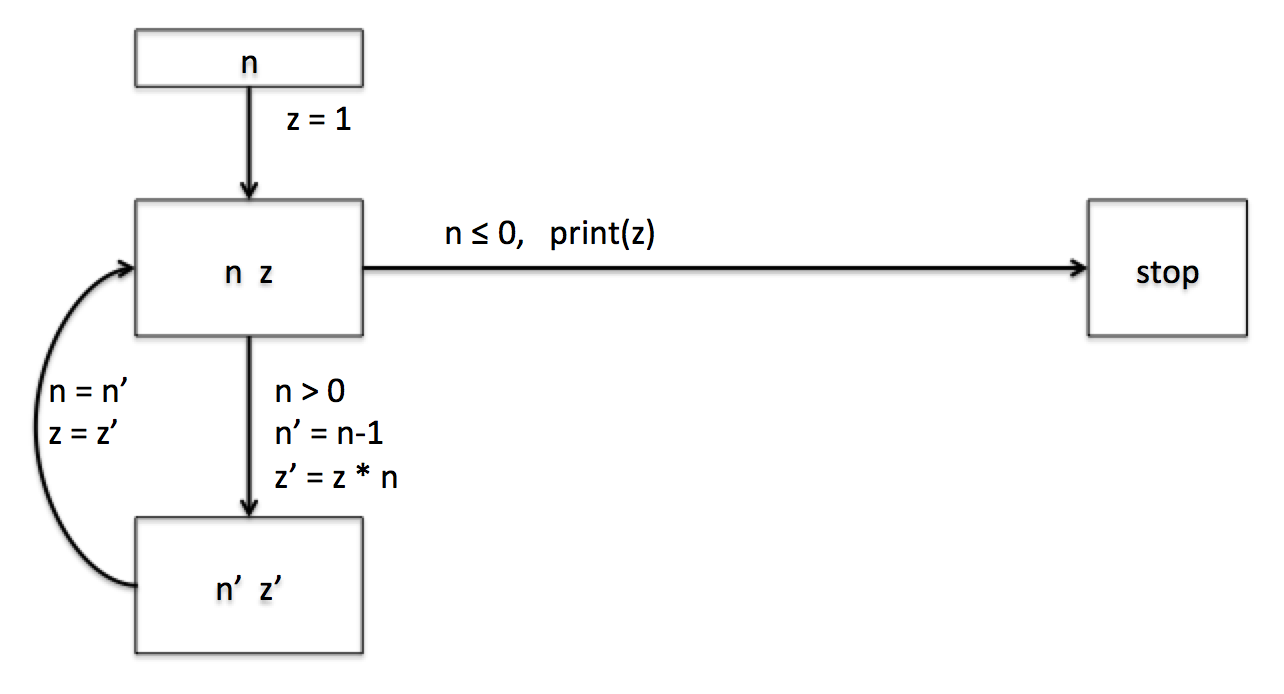
\includegraphics[width=7cm]{\figpath/transition-system}
    \end{center}
    \caption{}
  \end{subfigure}\\

  \caption{Transition system and constrained Horn clauses representing a program}
  \label{fig-horn}
\end{figure}

\begin{figure}
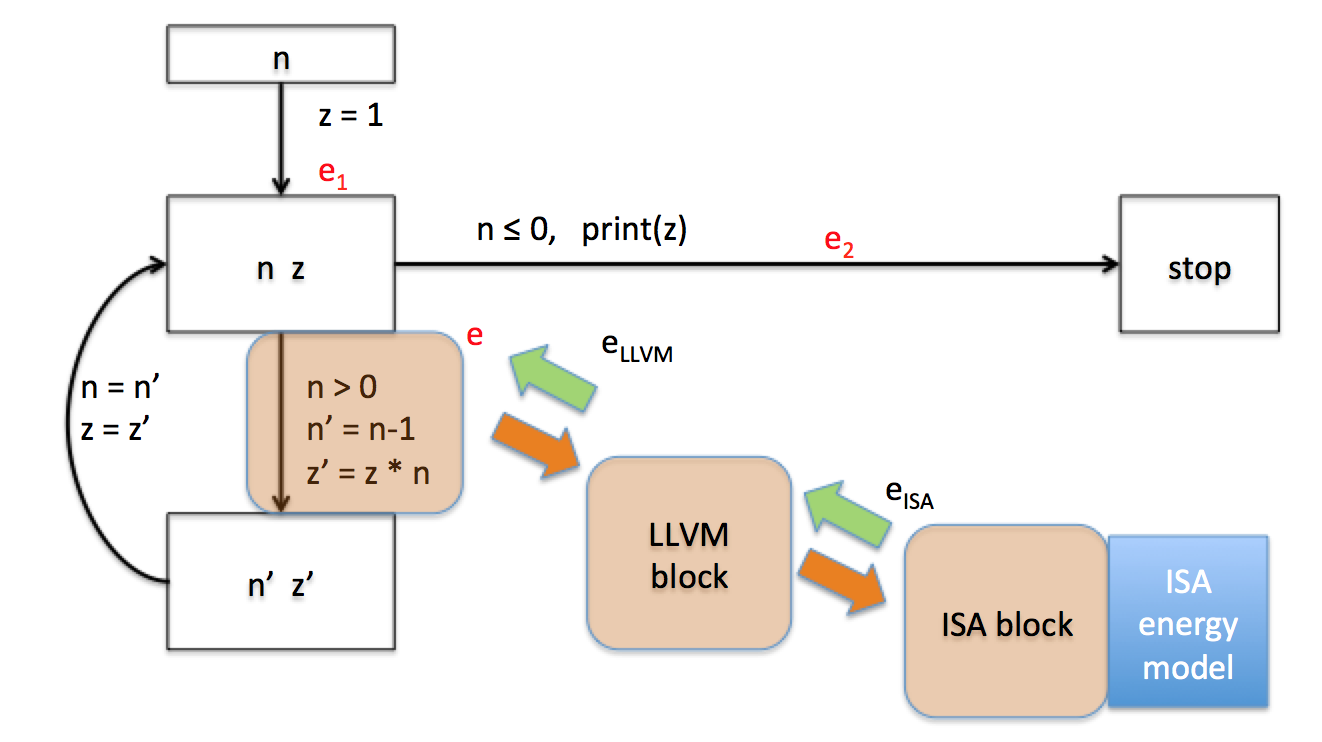
\includegraphics[width=8cm]{\figpath/mapping}   
 \caption{Combining an energy model with program analysis}
 \label{fig-model-mapping}
 \end{figure}

\subsection{Semantic representations of programs}
Code at various levels such as source code, intermediate compiler
representations or ISA needs to be translated into some suitable semantic
representation for analysis.   A common representation language is
constrained Horn clauses (CHCs), a subset of first order logic which is
widely used in software verification
\cite{DBLP:conf/birthday/BjornerGMR15}. CHCs can represent code at any
level of abstraction. A constrained Horn clause has the form $\forall x_0 \ldots x_n 
(p_1(x_1) \wedge \ldots \wedge p_n(x_N) \wedge \phi \rightarrow
p_0(x_0))$. When representing program semantics, each predicate
$p_0,p_1,\ldots,p_n$ typically corresponds to a program point, and its
respective arguments $x_0,x_1,\ldots,x_n$ are tuples representing the
state before and/or after those points.  A clause thus represents a
relationship between program states, and the constraint $\phi$ expresses
the relationship between the values of the state variables. A special case
of a Horn clause is where $n \le 1$, that is, there is at most one atomic
formula on the left of the clause.  Such a clause often represents a transition 
from the state at one program point to the next.

Figure \ref{fig-horn} illustrates the use of Horn clauses to 
represent an imperative program in a C-like language (a).
The constrained Horn clauses (b) represent a transition
system (c) induced by the program's semantics (the quantifiers in
the Horn clauses are
omitted).  The predicates
$r_0, \ldots, r_4$ represent the program points $1,\ldots,4$ and
$r_i(x_i)$ means that program point $i$  is reachable with state
$x_i$, where $x_i$ is the tuple of variables in scope at that point.

Lower-level programs such as ISA or intermediate code can be translated
in a similar fashion, where typically each predicate represents a basic block 
in the code. Semantics-based methods for translating sequential
imperative programs to
Horn clauses are explained in \cite{DBLP:conf/ppdp/AngelisFPP15}.
Furthermore techniques for representing multi-threaded
code as Horn clauses have been developed \cite{ GrebenshchikovLPR12}.

%
%
%Static analysis of energy consumption 
%gives safe approximations, namely upper and lower bounds, on the energy
%consumed by the program, or parts of it. These approximations are often
%functions parametrised by the sizes of the input data or contextual
%features such as clock frequency and voltage. 
%
%Static energy profiling~\cite{staticprofiling-flops} shows the
%distribution of energy usage over the parts of the code. This can be
%very useful to the developer, showing which parts of the program are the
%most energy-critical. Some functions or blocks in the program are
%perhaps not particularly expensive in energy in themselves but are
%called many times. Such parts are natural targets for optimisation,
%since there a small improvement can yield important savings. 

\subsection{Techniques for energy analysis}

Given such a representation of a program, techniques based on abstract interpretation \cite{Cousot1977}
can derive safe approximations of program behaviour. A branch of abstract interpretation 
focusses on automatic complexity analysis, yielding complexity functions on the
execution time of the program.  These techniques extend straightforwardly to analysis of energy and
other resources. The essence of the technique is to extract constraints from the Horn clauses
representing the energy consumed. These constraints are then solved, or approximated, to yield explicit 
formulas giving the consumption.


 
\paragraph{Linking analysis to an energy model.} The edges in the transition system can be 
associated with energy values, using an energy model. If the transition system is obtained
from the source code, then the energy model has to be mapped from a lower level model
such as an ISA model, possibly via an intermediate level as indicated in Figure \ref{fig-model-mapping}. 
Once this is done, constraints
representing the energy consumption of the program are extracted from the Horn clause 
representation. In the case of the loop at point 2, a recursive equation is obtained, e.g.
\[ cost_2(n) = e + cost_2(n-1)~ (\mathrm{if}~n\ge 0), ~~cost_2(n) = 0 ~ (\mathrm{if}~n < 0) \]
where $e$ is the energy cost of one iteration of the loop, obtained from the energy model. These
equations can be solved to yield the expression given the cost of the loop as a function of $n$, 
$cost_2(n) = n*e$, and the cost of the whole 
program (a path from 1 to 4) is $cost(n) = e_1 + n*e + e_2$, where $e_1, e_2$ are the respective
energy costs of the transitions before and after the loop.

\paragraph{More complex analyses.} The example shown is very simple, but the method generalises to
a wide range of program structures, including conditionals, next loops and procedure calls.  
As abstract interpretation is inherently approximate, the analysis in general gives safe upper and lower bounds on the energy
consumed by the program. 
A further extension of the method yields
static energy profiling~\cite{staticprofiling-flops}, which shows the
distribution of energy usage over the parts of the code, rather than a single function giving the total consumption of the program.
